\documentclass[12pt]{report}
\usepackage[utf8]{inputenc}
\usepackage[margin=1.2in]{geometry}
\usepackage{graphicx}
\usepackage{float}
\usepackage{subcaption}
\usepackage{amsmath}
\usepackage{amssymb}
\usepackage{ulem}
\usepackage{bm}
\usepackage{framed}
\usepackage{xcolor}
\usepackage{ragged2e}
\usepackage{color}
\usepackage{soul}
\usepackage{cancel}
\graphicspath{ {images/} }
\setlength{\parskip}{1em}
\allowdisplaybreaks


\usepackage{titling}
\newcommand{\subtitle}[1]{%
	\posttitle{%
		\par\end{center}
	\begin{center}\large#1\end{center}
	\vskip0.5em}%
}

\newenvironment{blueframed}[1][blue]
{\def\FrameCommand{\fboxsep=\FrameSep\fcolorbox{#1}{white}}%
\MakeFramed {\advance\hsize-\width \FrameRestore}}
{\endMakeFramed}

\newenvironment{spmatrix}[1]
{\def\mysubscript{#1}\mathop\bgroup\begin{bmatrix}}
	{\end{bmatrix}\egroup_{\textstyle\mathstrut\mysubscript}}

\title{Tutorial 10}
\subtitle
{
	\textbf{keywords}: time series, serial correlation, Breusch-Godfrey test, errors, residuals, dummy variables
	
	\textbf{estimated reading time}: 37 minutes
}
\author{Quang Bui}
\date{October 2, 2018}

\begin{document}
	
\maketitle

\section*{Question 1}
\noindent Excel file: \textit{SeattleElectric2005-06.xlxs} 

\noindent To open an Excel file with EViews,
$$Right\ click\ Excel\ file \to Open\ with \to EViews$$
\noindent \textit{SeattleElectric2005-06.xlxs} contains data on average hourly electricity usage in colds months in Seattle, USA, from 1 October 2005 to 31 March 2006. Information about each day during this time period is held in the following variables:
\begin{align*}
	date-&\ date\ in\ American\ format\ mm-dd-yyyy \\
	dow-&\ day\ of\ the\ week \\
	pubhol-&\ =1\ if\ that\ day\ was\ a\ public\ holiday, =0\ otherwise \\
	avetemp-&\ average\ daily\ temperature \\
	aveload-&\ average\ hourly\ electricity\ load\ on\ that\ day
\end{align*}
\vspace{-\baselineskip}
%%%%%%%%%% TABLE OBJECT %%%%%%%%%%
\begin{table}[H]
	\centering
	\begin{tabular}{lrrrrr}
		\multicolumn{1}{c}{}&\multicolumn{1}{r}{DATE}&\multicolumn{1}{r}{DOW}&\multicolumn{1}{r}{PUBHOL}&\multicolumn{1}{r}{AVETEMP}&\multicolumn{1}{r}{AVELOAD}\\
		\multicolumn{1}{c}{10/01/2005}&\multicolumn{1}{r}{$2005-10-01$}&\multicolumn{1}{r}{$7$}&\multicolumn{1}{r}{$0$}&\multicolumn{1}{r}{$63$}&\multicolumn{1}{r}{$1618$}\\
		\multicolumn{1}{c}{10/02/2005}&\multicolumn{1}{r}{$2005-10-02$}&\multicolumn{1}{r}{$1$}&\multicolumn{1}{r}{$0$}&\multicolumn{1}{r}{$60$}&\multicolumn{1}{r}{$1572$}\\
		\multicolumn{1}{c}{10/03/2005}&\multicolumn{1}{r}{$2005-10-03$}&\multicolumn{1}{r}{$2$}&\multicolumn{1}{r}{$0$}&\multicolumn{1}{r}{$55$}&\multicolumn{1}{r}{$1834$}\\
		\multicolumn{1}{c}{10/04/2005}&\multicolumn{1}{r}{$2005-10-04$}&\multicolumn{1}{r}{$3$}&\multicolumn{1}{r}{$0$}&\multicolumn{1}{r}{$59$}&\multicolumn{1}{r}{$1813$}\\
		\multicolumn{1}{c}{10/05/2005}&\multicolumn{1}{r}{$2005-10-05$}&\multicolumn{1}{r}{$4$}&\multicolumn{1}{r}{$0$}&\multicolumn{1}{r}{$58$}&\multicolumn{1}{r}{$1804$}\\
		\multicolumn{1}{c}{10/06/2005}&\multicolumn{1}{r}{$2005-10-06$}&\multicolumn{1}{r}{$5$}&\multicolumn{1}{r}{$0$}&\multicolumn{1}{r}{$58$}&\multicolumn{1}{r}{$1824$}\\
		\multicolumn{1}{c}{10/07/2005}&\multicolumn{1}{r}{$2005-10-07$}&\multicolumn{1}{r}{$6$}&\multicolumn{1}{r}{$0$}&\multicolumn{1}{r}{$55$}&\multicolumn{1}{r}{$1843$}\\
		\multicolumn{1}{c}{10/08/2005}&\multicolumn{1}{r}{$2005-10-08$}&\multicolumn{1}{r}{$7$}&\multicolumn{1}{r}{$0$}&\multicolumn{1}{r}{$55$}&\multicolumn{1}{r}{$1704$}\\
		\multicolumn{1}{c}{10/09/2005}&\multicolumn{1}{r}{$2005-10-09$}&\multicolumn{1}{r}{$1$}&\multicolumn{1}{r}{$0$}&\multicolumn{1}{r}{$57$}&\multicolumn{1}{r}{$1661$}\\
		\multicolumn{1}{c}{10/10/2005}&\multicolumn{1}{r}{$2005-10-10$}&\multicolumn{1}{r}{$2$}&\multicolumn{1}{r}{$1$}&\multicolumn{1}{r}{$58$}&\multicolumn{1}{r}{$1863$}\\
		\multicolumn{1}{c}{10/11/2005}&\multicolumn{1}{r}{$2005-10-11$}&\multicolumn{1}{r}{$3$}&\multicolumn{1}{r}{$0$}&\multicolumn{1}{r}{$57$}&\multicolumn{1}{r}{$1819$}\\
		\multicolumn{1}{c}{10/12/2005}&\multicolumn{1}{r}{$2005-10-12$}&\multicolumn{1}{r}{$4$}&\multicolumn{1}{r}{$0$}&\multicolumn{1}{r}{$57$}&\multicolumn{1}{r}{$1821$}\\
		\multicolumn{1}{c}{10/13/2005}&\multicolumn{1}{r}{$2005-10-13$}&\multicolumn{1}{r}{$5$}&\multicolumn{1}{r}{$0$}&\multicolumn{1}{r}{$57$}&\multicolumn{1}{r}{$1867$}\\
		\multicolumn{1}{c}{10/14/2005}&\multicolumn{1}{r}{$2005-10-14$}&\multicolumn{1}{r}{$6$}&\multicolumn{1}{r}{$0$}&\multicolumn{1}{r}{$56$}&\multicolumn{1}{r}{$1850$}\\
		\multicolumn{1}{c}{10/15/2005}&\multicolumn{1}{r}{$2005-10-15$}&\multicolumn{1}{r}{$7$}&\multicolumn{1}{r}{$0$}&\multicolumn{1}{r}{$58$}&\multicolumn{1}{r}{$1724$}\\
	\end{tabular}
	\caption{Data for the first 15 days during the cold months in Seattle, USA, October 2005 to March 2006.}
	%\label{tab:}
\end{table} \centering $dow=7:\ Saturday,\ dow=1:\ Sunday,\ dow=2:\ Monday,\ \dots\ ,  dow=6:\ Friday$


\newpage
\justify \noindent \textcolor{red}
{
	(a) Use $dow$ to create dummy variables for different days of the week. Especially, create dummy variables for Saturday and Sunday and also a dummy variable called $wknd$ which is 1 if the day is a Saturday or a Sunday, and 0 for any other day.
}
\begin{equation*}
	sat_i = \begin{cases}
		1 & if\ i^{th}\ day\ is\ a\ Saturday \\
		0 & otherwise
	\end{cases}
\end{equation*}
\begin{equation*}
	sun_i = \begin{cases}
	1 & if\ i^{th}\ day\ is\ a\ Sunday \\
	0 & otherwise
	\end{cases}
\end{equation*}
\noindent To create the Saturday dummy variables using $dow$,
$$EViews\ Command\ window: series\ sat=(dow=7)$$
\begin{figure}[H]
	\centering
	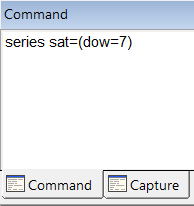
\includegraphics{q1_1}
\end{figure} \vspace{-\baselineskip} \centering $(Press\ Enter\ to\ execute\ code)$

\justify \noindent To create the Sunday dummy variables using $dow$,
$$EViews\ Command\ window: series\ sun=(dow=1)$$
\begin{figure}[H]
	\centering
	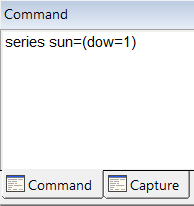
\includegraphics{q1_2}
\end{figure} \vspace{-\baselineskip} \centering $(Press\ Enter\ to\ execute\ code)$
\justify \noindent Using $sat$ and $sun$, create the dummy variable $wknd$,
\begin{equation*}
	wknd_i = \begin{cases}
	1 & if\ i^{th}\ day\ is\ a\ weekend \\
	0 & otherwise
	\end{cases}
\end{equation*}
\begin{figure}[H]
	\centering
	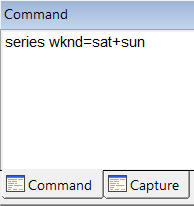
\includegraphics{q1_3}
\end{figure}
\vspace{-\baselineskip}
\begin{figure}[H]
	\centerline{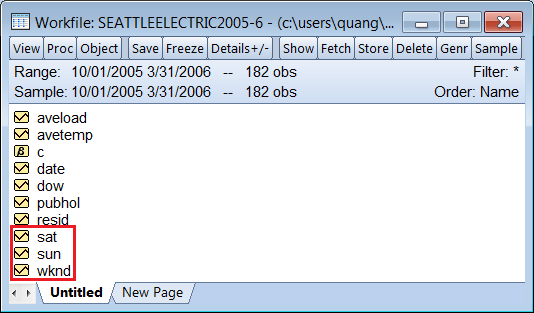
\includegraphics{tute9_1}}
\end{figure}
\vspace{-\baselineskip}
\begin{figure}[H]
	\centerline{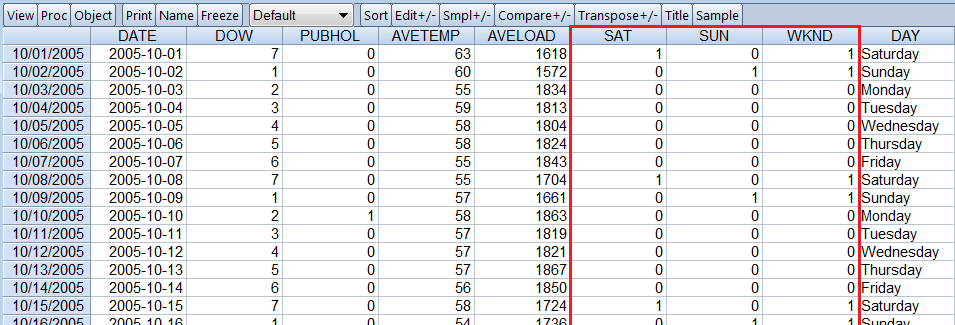
\includegraphics{q1_4}}
\end{figure}

\newpage
\noindent \textcolor{red}
{
	(b) The goal is to predict $aveload$ in winter months (Seattle, USA, is in the Northern hemisphere) based on temperature and other available information (our assumption is that the weather bureau can produce temperature forecasts that are pretty accurate). Given this goal, have an appropriate look at the data. In particular, investigate differences in average load in different days of the week and look at the scatter plot of $aveload$ against $avetemp$ to familiarise yourself with the data. \\ \\ Remember that a good analyst does not confine himself or herself to any particular software. If a pivot chart would be better for visualising differences in average load in difference days of the week, then use it! If you have learnt another software (for example R, SPSS or STATA) in another unit that you think will be more helpful, use it!
}

\noindent \uline{Investigate the difference in average hourly electricity load in different days of the week}

\noindent We can produce a column graph of the average of $aveload$ for each day of the week using Excel’s Pivot Chart. To produce the Pivot Chart, select any cell in the data set then,
$$Insert \to PivotTable \to OK$$
\begin{figure}[H]
	\centerline{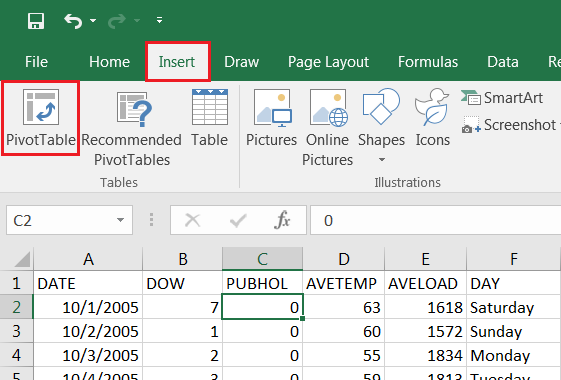
\includegraphics{q1_5}}
\end{figure}
\vspace{-\baselineskip}
\begin{figure}[H]
	\centerline{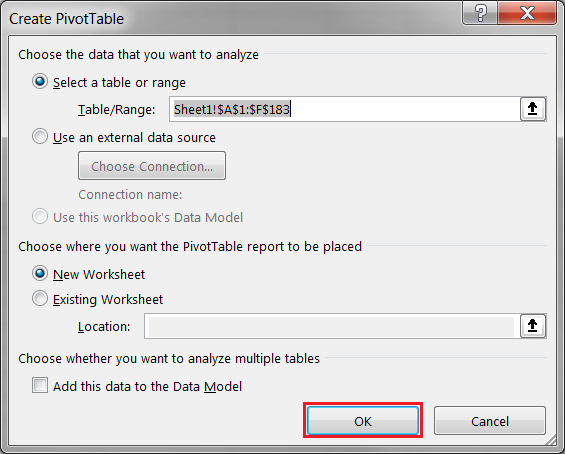
\includegraphics{q1_6}}
\end{figure}
\vspace{-\baselineskip}
\noindent From the PivotTable Fields, drag and drop $day$ and $aveload$ into the Row and Value windows respectively,
\begin{figure}[H]
	\centerline{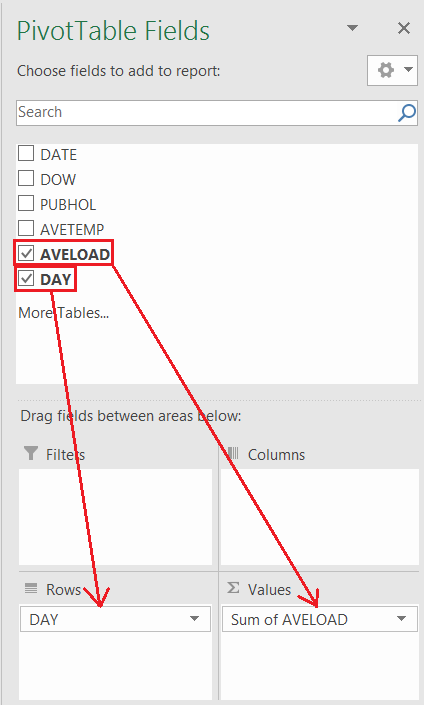
\includegraphics{q1_7}}
\end{figure}
\vspace{-\baselineskip}
\noindent We want the mean of the average hourly electricity load for each day in the Pivot Table,
\begin{align*}
	\overline{average\ Monday\ hourly\ electricity\ load} &= \dfrac{\sum average\ Monday\ hourly\ electricity\ load}{no.\ of\ Mondays\ in\ sample} \\
	\overline{average\ Tuesday\ hourly\ electricity\ load} &= \dfrac{\sum average\ Tuesday\ hourly\ electricity\ load}{no.\ of\ Tuesdays\ in\ sample} \\
	\vdots \\
	\overline{average\ Sunday\ hourly\ electricity\ load} &= \dfrac{\sum average\ Sunday\ hourly\ electricity\ load}{no.\ of\ Sundays\ in\ sample}
\end{align*}

\newpage
\noindent To do this, change the Summarised Value of $avetemp$ from Sum to Average. Click the drop-down arrow,
\begin{figure}[H]
	\centerline{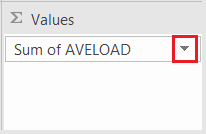
\includegraphics{q1_8}}
\end{figure}
\vspace{-\baselineskip}
$$Value\ Field\ Settings \to Average \to OK$$
\begin{figure}[H]
	\centerline{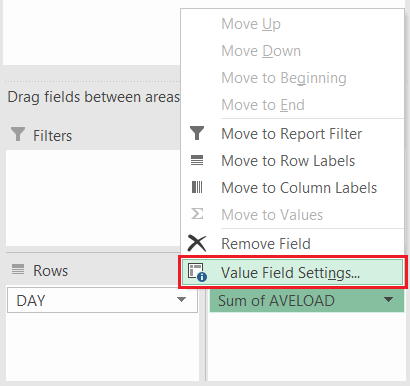
\includegraphics{q1_9}}
\end{figure}
\vspace{-\baselineskip}
\begin{figure}[H]
	\centerline{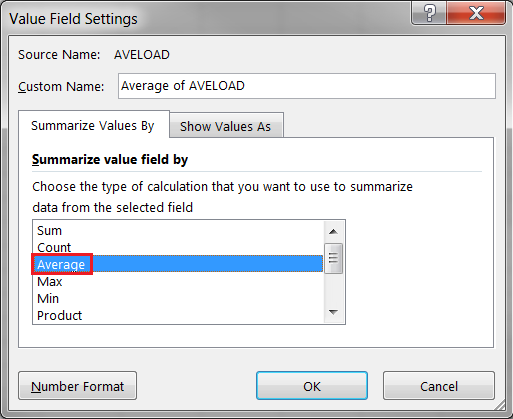
\includegraphics{q1_10}}
\end{figure}
\vspace{-\baselineskip}
\noindent To automatically name the PivotChart headings with variables names,
$$Design \to Report\ Layout \to Show\ in\ Tabular\ Form$$
\begin{figure}[H]
	\centerline{
\includegraphics{q1_11}}
\end{figure}
\vspace{-\baselineskip}

\newpage
\noindent To produce a column graph from the Pivot Table,
$$Analyze \to PivotChart \to Clustered\ Column \to OK$$
\begin{figure}[H]
	\centerline{
\includegraphics{q1_12}}
\end{figure}
\vspace{-\baselineskip}
\begin{figure}[H]
	\centerline{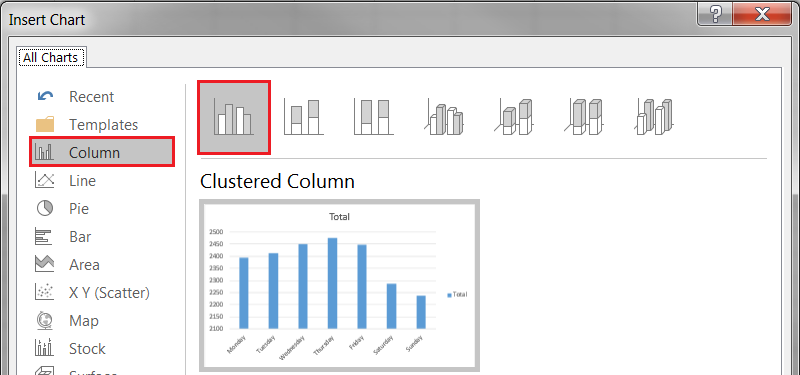
\includegraphics{q1_13}}
\end{figure}
\vspace{-\baselineskip}
\begin{figure}[H]
	\centerline{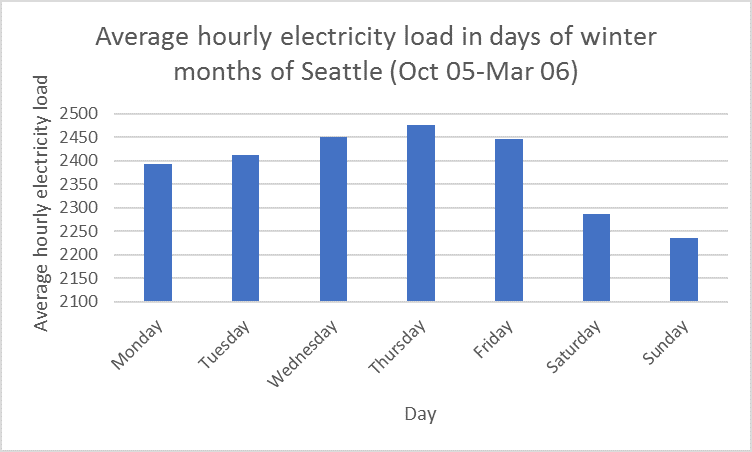
\includegraphics{q1_14}}
\end{figure}
\vspace{-\baselineskip}
\noindent From the Pivot Chart, we find that, on average, electricity load during the winter months of Seattle is lowest during the weekends.

\noindent \uline{Investigate the relationship between average hourly electricity load and average daily temperature}

\noindent Produce a scatter plot of $aveload$ against $avetemp$,
$$Quick \to Graph \to avetemp\ aveload \to Specific: Scatter \to OK$$
\begin{figure}[H]
	\centerline{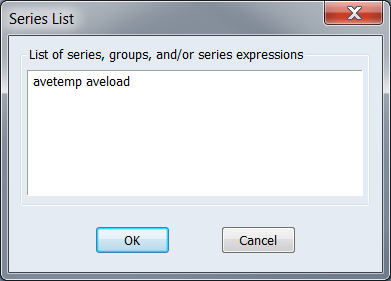
\includegraphics{q1_15}}
\end{figure}
\vspace{-\baselineskip}
\begin{figure}[H]
	\centerline{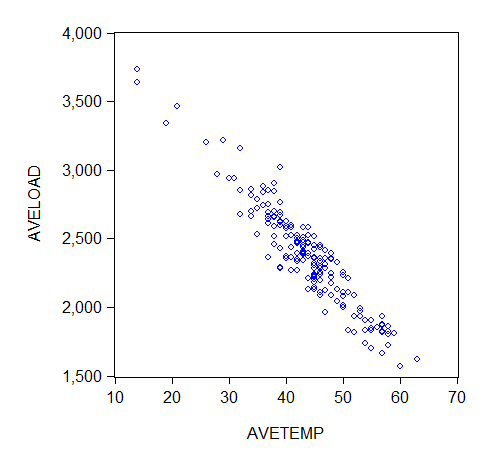
\includegraphics{q1_16}}
\end{figure}
\vspace{-\baselineskip}
\noindent The scatter plot suggests a strong negative linear relationship between average hourly electricity load and average daily temperature. During the days of the winter months, as average temperate increases, electricity load decreases.

\newpage
\noindent \textcolor{red}
{
	(c) Estimate a regression of $aveload$ on a constant, $avetemp$, $wknd$ and public holiday dummies, $$aveload_t = \beta_0 + \beta_1 avetemp_t + \beta_2wknd_t + \beta_3pubhol_t + u_t$$
}
\noindent To estimate the model of average hourly electricity load from the Command Window in EViews,
\begin{figure}[H]
	\centerline{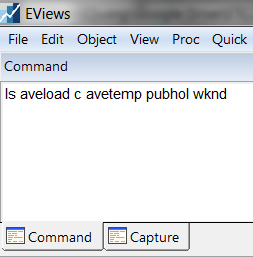
\includegraphics{tute10_1}}
\end{figure}
\vspace{-\baselineskip}
%%%%%%%%%% TABLE OBJECT %%%%%%%%%%
\begin{table}[H]
	\centering
	\begin{tabular}{lrrrr}
		\multicolumn{3}{l}{Dependent Variable: AVELOAD}&\multicolumn{1}{c}{}&\multicolumn{1}{c}{}\\
		\multicolumn{3}{l}{Method: Least Squares}&\multicolumn{1}{c}{}&\multicolumn{1}{c}{}\\
		\multicolumn{3}{l}{Sample: 10/01/2005 3/31/2006}&\multicolumn{1}{c}{}&\multicolumn{1}{c}{}\\
		\multicolumn{3}{l}{Included observations: 182}&\multicolumn{1}{c}{}&\multicolumn{1}{c}{}\\
		[4.5pt] \hline \\ [-4.5pt]
		\multicolumn{1}{c}{Variable}&\multicolumn{1}{r}{Coefficient}&\multicolumn{1}{r}{Std. Error}&\multicolumn{1}{r}{t-Statistic}&\multicolumn{1}{r}{Prob.}\\
		[4.5pt] \hline \\ [-4.5pt]
		\multicolumn{1}{c}{C}&\multicolumn{1}{r}{$4332.783$}&\multicolumn{1}{r}{$41.79892$}&\multicolumn{1}{r}{$103.6578$}&\multicolumn{1}{r}{$0.0000$}\\
		\multicolumn{1}{c}{AVETEMP}&\multicolumn{1}{r}{$-43.58037$}&\multicolumn{1}{r}{$0.940259$}&\multicolumn{1}{r}{$-46.34931$}&\multicolumn{1}{r}{$0.0000$}\\
		\multicolumn{1}{c}{PUBHOL}&\multicolumn{1}{r}{$-121.5734$}&\multicolumn{1}{r}{$31.00930$}&\multicolumn{1}{r}{$-3.920546$}&\multicolumn{1}{r}{$0.0001$}\\
		\multicolumn{1}{c}{WKND}&\multicolumn{1}{r}{$-143.6717$}&\multicolumn{1}{r}{$16.35973$}&\multicolumn{1}{r}{$-8.782032$}&\multicolumn{1}{r}{$0.0000$}\\
		[4.5pt] \hline \\ [-4.5pt]
		\multicolumn{1}{l}{R-squared}&\multicolumn{1}{r}{$0.927222$}&\multicolumn{2}{l}{Mean dependent var}&\multicolumn{1}{r}{$2386.005$}\\
		\multicolumn{1}{l}{Adjusted R-squared}&\multicolumn{1}{r}{$0.925995$}&\multicolumn{2}{l}{S.D. dependent var}&\multicolumn{1}{r}{$365.8870$}\\
		\multicolumn{1}{l}{S.E. of regression}&\multicolumn{1}{r}{$99.53527$}&\multicolumn{2}{l}{Akaike info criterion}&\multicolumn{1}{r}{$12.06063$}\\
		\multicolumn{1}{l}{Sum squared resid}&\multicolumn{1}{r}{$1763494.$}&\multicolumn{2}{l}{Schwarz criterion}&\multicolumn{1}{r}{$12.13105$}\\
		\multicolumn{1}{l}{Log likelihood}&\multicolumn{1}{r}{$-1093.518$}&\multicolumn{2}{l}{Hannan-Quinn criter.}&\multicolumn{1}{r}{$12.08918$}\\
		\multicolumn{1}{l}{F-statistic}&\multicolumn{1}{r}{$755.9290$}&\multicolumn{2}{l}{Durbin-Watson stat}&\multicolumn{1}{r}{$0.942970$}\\
		\multicolumn{1}{l}{Prob(F-statistic)}&\multicolumn{1}{r}{$0.000000$}&\multicolumn{1}{c}{}&\multicolumn{1}{c}{}&\multicolumn{1}{c}{}\\
		[4.5pt] \hline \\ [-4.5pt]
	\end{tabular}
	$$\widehat{aveload}_t = \underset{(41.7990)}{4332.783} - \underset{(0.9403)}{43.5804}avetemp_t - \underset{(16.3597)}{143.6717}wknd_t - \underset{(31.0093)}{121.5734}pubhol_t$$
\end{table}

\noindent \textcolor{red}{We know that electricity usage, like anything else in life, is likely to be related to what the usage was in previous days. 
	\begin{align*}
	corr(aveload_t, aveload_{t-1}) &\neq 0 \\
	corr(aveload_t, aveload_{t-2}) &\neq 0 \\
	\vdots  
	\end{align*}
	As a result, we suspect that part of the electricity load that cannot be explained by temperature, $$u_t$$ is likely to be correlated over time,
	\begin{align*}
	corr(u_t, u_{t-1}) &\neq 0 \\
	corr(u_t, u_{t-2}) &\neq 0 \\
	\vdots 
	\end{align*}} \vspace{-\baselineskip}

\noindent This is because
\begin{align*}
	aveload_t &= \beta_0 + \beta_1 avetemp_t + \beta_2wknd_t + \beta_3pubhol_t + u_t \\
	aveload_{t-1} &= \beta_0 + \beta_1 avetemp_{t-1} + \beta_2wknd_{t-1} + \beta_3pubhol_{t-1} + u_{t-1} \\
	aveload_{t-2} &= \beta_0 + \beta_1 avetemp_{t-2} + \beta_2wknd_{t-2} + \beta_3pubhol_{t-2} + u_{t-2} \\
	&\vdots
\end{align*} \noindent When the errors are correlated with itself over different time periods, we say that the errors are serially correlated.

\noindent \textcolor{red}{If that is the case, what consequences would that have for the OLS estimator? In such a case, can we use the model that you estimated to test that there is no difference in the intercept in weekdays and weekends?}




\justify
\begin{blueframed}
	\textcolor{blue}{\textbf{Background}}
	\vspace{-\baselineskip}
	\justify
	\textcolor{blue}{\underline{Consequences of serially correlated errors (autocorrelated errors)}}
	
	\noindent \textcolor{blue}
	{
		When the assumption of serially uncorrelated errors is violated, the OLS estimator remains unbiased (if the unbiasedness assumptions hold) but will no longer be the most efficient unbiased estimator. More importantly, the OLS standard errors will be incorrect, and the t and F test-statistic will not follow a t and F distribution, even asymptotically.
	}
\end{blueframed}
\begin{itemize}
	\item The OLS estimator of the parameters in our model of $aveload$ is unbiased but no longer the most efficient unbiased estimator.
	\item Cannot use our estimated model of average hourly electricity load to test if there is a difference in intercept between weekdays and weekends.
\end{itemize}



\newpage
\noindent \textcolor{red}
{
	(d) Use visual aids and a formal test to test the hypothesis that errors of this model are white noise against the alternative that they are generated by an AR(7). You should reject the null. Then investigate what kind of AR model would be sufficient for capturing the dynamics of the errors (the t-statistics in your BG auxiliary regression may give you a hint, and the partial autocorrelations of the residuals in the correlogram are informative as well). Re-estimate the model by adding an AR equation for $u_t$.
}

\justify
\begin{blueframed}
	\textcolor{blue}{\textbf{Background}}
	\vspace{-\baselineskip}
	\justify
	\textcolor{blue}{\underline{Residuals and Errors}}
	
	\noindent \textcolor{blue}
	{
		The residuals is the difference between the observed average hourly electricity load and the predicted/fitted average hourly electricity load, 
		$$\hat{u}_1 = aveload_1 - \widehat{aveload}_1$$
		$$\hat{u}_2 = aveload_2 - \widehat{aveload}_2$$
		$$\vdots$$
		$$\hat{u}_n = aveload_n - \widehat{aveload}_n$$
		\noindent Although the errors are unobserved, the residuals are observed. This means that we can obtain a line graph or the correlogram of the residuals to determine if there is evidence of serial correlation. Furthermore, we can formally test for serial correlation in the unobserved errors by performing a test on the observed residuals. \\ \\ \uline{White Noise} \\ \\
		If the errors are white noise, then they are serially uncorrelated $$corr({u}_t, {u}_{t-j}) = 0 \qquad for\ all\ j\ except\ j=0$$ and its expectation equals to 0 and variance is constant (but unknown), \begin{align*}
			E({u}_t) &= 0 \\
			Var({u}_t) &= \sigma^2
		\end{align*} \vspace{-\baselineskip}
	}
\end{blueframed}

\noindent \uline{Visual aid to determine if the errors are white noise or serially correlated}

\noindent Since we cannot plot a line graph of the errors (because they are unobserved) to determine if there is presence of serial correlation in the errors, we instead plot a line graph of the residuals.

\noindent If the residuals follow a pattern, this suggests that the errors are serially correlated. On the other hand, a residual plot that does not exhibit any patterns i.e. one that looks like white noise would suggest that the errors are not serially correlated.

\noindent To obtain a line graph of $aveload$, $\widehat{aveload}$, and $\hat{u}$ from the estimated model of $aveload$ in EViews (I have named the equation $eq01$ in EViews), $$eq01 \to View\ \to Actual,Fitted,Residual \to Residual\ Graph$$
\begin{figure}[H]
	\centerline{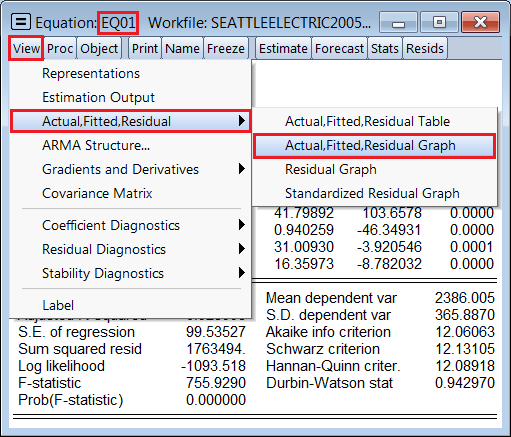
\includegraphics{tute10_2}}
\end{figure}
\vspace{-\baselineskip}
\begin{figure}[H]
	\centerline{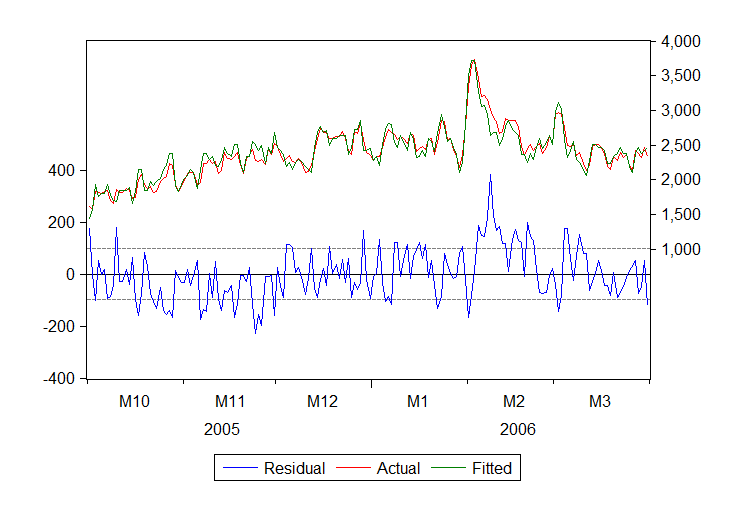
\includegraphics{tute10_3}}
\end{figure}
\vspace{-\baselineskip} \noindent The line graph of the residuals shows there is a slight cyclical pattern i.e.positive residuals are likely followed by positive residuals and negative residuals are likely followed by negative residuals. This indicates that there error is positively serially correlated. 

\noindent After visually inspecting the residual plot, we should formally test for serially correlated errors.


\newpage
\justify
\begin{blueframed}
	\textcolor{blue}{\textbf{Background}}
	\vspace{-\baselineskip}
	\justify
	\textcolor{blue}{\underline{Breusch-Godfrey test for serial correlation in the errors}}
	
	\noindent \textcolor{blue}
	{
		Since we are testing for serial correlation in $u_t$ of order 7, our model of $aveload$ is
		\begin{align}
		aveload_t &= \beta_0 + \beta_1 avetemp_t + \beta_2wknd_t + \beta_3pubhol_t + u_t \\
		u_t &= \rho_1u_{t-1} + \rho_2u_{t-2} + \rho_3u_{t-3} + \dots + \rho_7u_{t-7} + e_t
		\end{align} $$\{e_t, t=1,2,\dots,n \sim i.i.d(0,\sigma^2)\}$$ where $e_t$ for $t=1,2,\dots,n$ are independent and identically distributed with mean 0 and variance $\sigma^2$ (which means that $e_t$ for $t=1,2,\dots,n$ are unrelated to each other and have equal variance i.e. homoskedastic and serially uncorrelated). \\ \\
		\noindent The null and alternative hypothesis can be written as:
		\begin{align*}
		H_0&: \rho_1 = \rho_2 = \rho_3 = \dots = \rho_7 = 0 \\
		H_1&: at\ least\ one\ of\ the\ 7\ autoregressive\ parameters\ \neq\ 0
		\end{align*} Since we do not observe $u_t$, we cannot estimate equation (2) and test the above hypothesis. \\ \\
		To perform the Breusch-Godfrey test for serial correlation in the errors of model of $aveload$ at any lag up to and include lag 7 (7th order serial correlation),
		\begin{itemize}
			\item Estimate the model of $aveload$ (equation (1))
			\item Save the residuals from the estimated model of $aveload$
			\item Then estimate the following $auxiliary\ regression \dots$ $$\hat{u}_t = \alpha_0 + \alpha_1avetemp + \alpha_2wknd + \alpha_3pubhol + \rho_1\hat{u}_{t-1} + \rho_2\hat{u}_{t-2} + \dots + \rho_7\hat{u}_{t-7} + v_t$$
			\item We're testing the null hypothesis that there is no serial correlation in the errors at any lag up to and include lag 7, against the alternative hypothesis that there is serial correlation in the errors in at least one lag up to and including lag 7.
			\item Compare the calculated test statistics with the critical value and conclude if there is evidence of serial correlation in the errors in at least one lag up to and including lag 7.
		\end{itemize}
		\noindent There are two forms of the Breusch-Godfrey test (both are only valid asymptotically):
	}
\end{blueframed}

\justify
\begin{blueframed}
	\vspace{-\baselineskip}
	
	\noindent \textcolor{blue}
	{
		\begin{itemize}
			\item The first form uses the F test statistic, $$F = \dfrac{(SSR_r - SSR_{ur})/q}{SSR_{ur}/(n-k-1)} \overset{asy}{\sim} F_{q,n-k-1} \quad under\ H_0$$
			\item The second form uses the BG test statistic, $$BG = (n-q)\times R^2_{\hat{u}} \overset{asy}{\sim} \chi^2_q \quad under\ H_0$$
		\end{itemize}
		\noindent where $q=7$ represents the orders of lag that we are testing. \\ \\ Note: In the BG test statistic, $q$ is subtracted from $n$ because we lose $q$ observations when we include $q$ lags of the residuals in the auxiliary regression.
	}
\end{blueframed}





\noindent To perform the Breusch-Godfrey test for 7th order serial correlation in the errors, generate the residuals from the estimated model of $aveload$, $$eq01 \to Proc \to Make\ Residual\ Series$$
\begin{figure}[H]
	\centerline{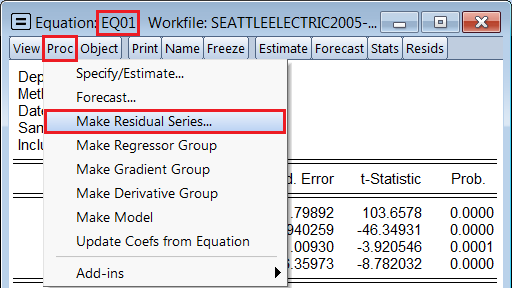
\includegraphics{tute10_4}}
\end{figure}
\vspace{-\baselineskip} \noindent and name the residual series $uhat$,
\begin{figure}[H]
	\centerline{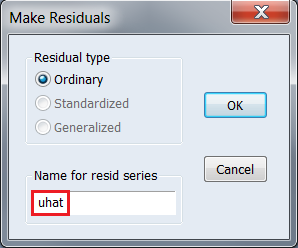
\includegraphics{tute10_5}}
\end{figure}
\vspace{-\baselineskip} \noindent then estimated the following auxiliary regression, $$\hat{u}_t = \alpha_0 + \alpha_1avetemp + \alpha_2wknd + \alpha_3pubhol + \rho_1\hat{u}_{t-1} + \rho_2\hat{u}_{t-2} + \dots + \rho_7\hat{u}_{t-7} + v_t$$ $$uhat\ c\ avetemp\ wknd\ pubhol\ uhat(-1to-7)$$ \begin{figure}[H]
	\centerline{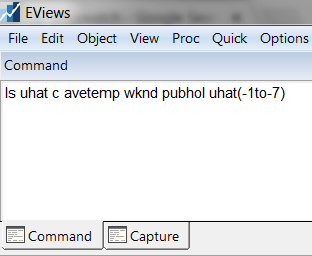
\includegraphics{tute10_6}}
\end{figure}
\vspace{-\baselineskip}
%%%%%%%%%% TABLE OBJECT %%%%%%%%%%
\begin{table}[H]
	\centering
	\begin{tabular}{lrrrr}
		\multicolumn{3}{l}{Dependent Variable: UHAT}&\multicolumn{1}{c}{}&\multicolumn{1}{c}{}\\
		\multicolumn{3}{l}{Method: Least Squares}&\multicolumn{1}{c}{}&\multicolumn{1}{c}{}\\
		\multicolumn{4}{l}{Sample (adjusted): 10/08/2005 3/31/2006}&\multicolumn{1}{c}{}\\
		\multicolumn{5}{l}{Included observations: 175 after adjustments}\\
		[4.5pt] \hline \\ [-4.5pt]
		\multicolumn{1}{c}{Variable}&\multicolumn{1}{r}{Coefficient}&\multicolumn{1}{r}{Std. Error}&\multicolumn{1}{r}{t-Statistic}&\multicolumn{1}{r}{Prob.}\\
		[4.5pt] \hline \\ [-4.5pt]
		\multicolumn{1}{c}{C}&\multicolumn{1}{r}{$-25.17570$}&\multicolumn{1}{r}{$38.59715$}&\multicolumn{1}{r}{$-0.652268$}&\multicolumn{1}{r}{$0.5151$}\\
		\multicolumn{1}{c}{AVETEMP}&\multicolumn{1}{r}{$0.537992$}&\multicolumn{1}{r}{$0.883942$}&\multicolumn{1}{r}{$0.608628$}&\multicolumn{1}{r}{$0.5436$}\\
		\multicolumn{1}{c}{WKND}&\multicolumn{1}{r}{$-0.186538$}&\multicolumn{1}{r}{$14.09467$}&\multicolumn{1}{r}{$-0.013235$}&\multicolumn{1}{r}{$0.9895$}\\
		\multicolumn{1}{c}{PUBHOL}&\multicolumn{1}{r}{$30.10940$}&\multicolumn{1}{r}{$26.60905$}&\multicolumn{1}{r}{$1.131547$}&\multicolumn{1}{r}{$0.2595$}\\
		\multicolumn{1}{c}{UHAT(-1)}&\multicolumn{1}{r}{$0.493938$}&\multicolumn{1}{r}{$0.079677$}&\multicolumn{1}{r}{$6.199229$}&\multicolumn{1}{r}{$0.0000$}\\
		\multicolumn{1}{c}{UHAT(-2)}&\multicolumn{1}{r}{$0.003029$}&\multicolumn{1}{r}{$0.087706$}&\multicolumn{1}{r}{$0.034533$}&\multicolumn{1}{r}{$0.9725$}\\
		\multicolumn{1}{c}{UHAT(-3)}&\multicolumn{1}{r}{$-0.008167$}&\multicolumn{1}{r}{$0.086885$}&\multicolumn{1}{r}{$-0.094002$}&\multicolumn{1}{r}{$0.9252$}\\
		\multicolumn{1}{c}{UHAT(-4)}&\multicolumn{1}{r}{$0.108065$}&\multicolumn{1}{r}{$0.086073$}&\multicolumn{1}{r}{$1.255496$}&\multicolumn{1}{r}{$0.2111$}\\
		\multicolumn{1}{c}{UHAT(-5)}&\multicolumn{1}{r}{$0.153122$}&\multicolumn{1}{r}{$0.086524$}&\multicolumn{1}{r}{$1.769712$}&\multicolumn{1}{r}{$0.0786$}\\
		\multicolumn{1}{c}{UHAT(-6)}&\multicolumn{1}{r}{$0.014457$}&\multicolumn{1}{r}{$0.087593$}&\multicolumn{1}{r}{$0.165050$}&\multicolumn{1}{r}{$0.8691$}\\
		\multicolumn{1}{c}{UHAT(-7)}&\multicolumn{1}{r}{$-0.061279$}&\multicolumn{1}{r}{$0.078089$}&\multicolumn{1}{r}{$-0.784737$}&\multicolumn{1}{r}{$0.4337$}\\
		[4.5pt] \hline \\ [-4.5pt]
		\multicolumn{1}{l}{R-squared}&\multicolumn{1}{r}{$0.340335$}&\multicolumn{2}{l}{Mean dependent var}&\multicolumn{1}{r}{$-0.266614$}\\
		\multicolumn{1}{l}{Adjusted R-squared}&\multicolumn{1}{r}{$0.300112$}&\multicolumn{2}{l}{S.D. dependent var}&\multicolumn{1}{r}{$99.16426$}\\
		\multicolumn{1}{l}{S.E. of regression}&\multicolumn{1}{r}{$82.96015$}&\multicolumn{2}{l}{Akaike info criterion}&\multicolumn{1}{r}{$11.73539$}\\
		\multicolumn{1}{l}{Sum squared resid}&\multicolumn{1}{r}{$1128711.$}&\multicolumn{2}{l}{Schwarz criterion}&\multicolumn{1}{r}{$11.93432$}\\
		\multicolumn{1}{l}{Log likelihood}&\multicolumn{1}{r}{$-1015.847$}&\multicolumn{2}{l}{Hannan-Quinn criter.}&\multicolumn{1}{r}{$11.81608$}\\
		\multicolumn{1}{l}{F-statistic}&\multicolumn{1}{r}{$8.461108$}&\multicolumn{2}{l}{Durbin-Watson stat}&\multicolumn{1}{r}{$1.928231$}\\
		\multicolumn{1}{l}{Prob(F-statistic)}&\multicolumn{1}{r}{$0.000000$}&\multicolumn{1}{c}{}&\multicolumn{1}{c}{}&\multicolumn{1}{c}{}\\
		[4.5pt] \hline \\ [-4.5pt]
	\end{tabular}
	%$$n_{aux} = n - q = 182 - 7 = 175$$ $$R^2_{aux} = 0.3403$$
	%\label{tab:}
\end{table}
\vspace{-\baselineskip} $$n_{aux} = n - q = 182 - 7 = 175 \qquad R^2_{aux} = 0.3403$$
\noindent Auxiliary regression: $$\hat{u}_t = \alpha_0 + \alpha_1avetemp + \alpha_2wknd + \alpha_3pubhol + \rho_1\hat{u}_{t-1} + \rho_2\hat{u}_{t-2} + \dots + \rho_7\hat{u}_{t-7} + v_t$$ 
\noindent Estimated auxiliary regression: \begin{align*}
	\widehat{\hat{u}}_t &= -25.1757 + 0.5380avetemp -0.1866wknd + 30.1094pubhol + 0.4939\hat{u}_{t-1} \\ 
	&+ 0.0030\hat{u}_{t-2} + \dots - 0.0613\hat{u}_{t-7} + v_t
\end{align*} 
\noindent BG test statistic: 
$$BG = (n-7)\times R^2_{\hat{u}} \overset{asy}{\sim} \chi^2_7 \quad under\ H_0$$
\noindent Calculate BG test statistic: 
$$BG_{calc} = 175\times 0.3403 = 59.5525$$
\noindent Critical value: 
\begin{figure}[H]
	\centerline{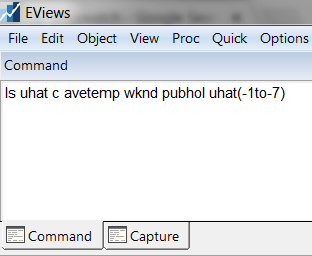
\includegraphics{tute10_6}}
\end{figure}
\vspace{-\baselineskip}
\begin{figure}[H]
	\centerline{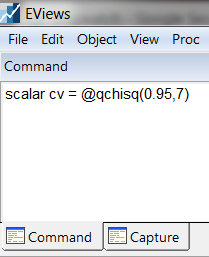
\includegraphics{tute10_7}}
\end{figure}
\vspace{-\baselineskip}
\begin{figure}[H]
	\centerline{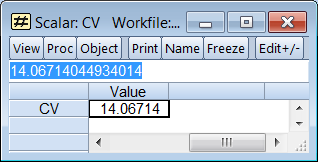
\includegraphics{tute10_8}}
\end{figure}
\vspace{-\baselineskip}
$$BG_{crit} = 14.0671$$

\noindent Since $BG_{calc}= 59.5525 > BG_{crit} = 14.0671$ we reject the null and conclude that there is sufficient evidence from our sample to suggesting that there is serial correlation in the errors in at least one lag up to and include the 7th lag.

\noindent \uline{Investigate what kind of AR model would be sufficient for capturing the dynamics of the errors (the t-statistics in your BG auxiliary regression may give you a hint, and the partial autocorrelations of the residuals in the correlogram are informative as well).}

\noindent To obtain the correlogram of the residuals of the estimated model of $aveload$, $$eq01 \to View \to Residual\ Diagnostics \to Correlogram\ Q-statistics$$
\begin{figure}[H]
	\centerline{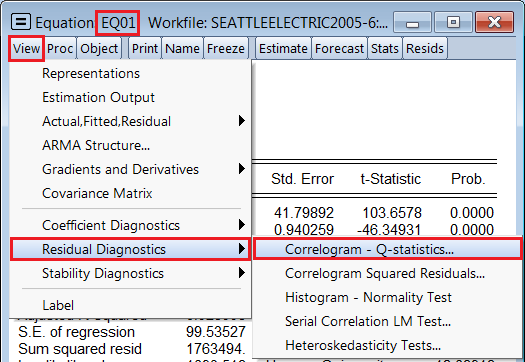
\includegraphics{tute10_10}}
\end{figure}
\vspace{-\baselineskip}$$Lags\ to\ include:36$$

\begin{figure}[H]
	\centerline{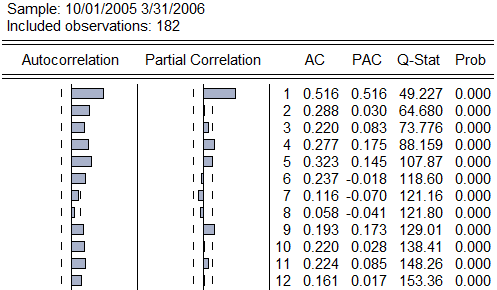
\includegraphics{tute10_9}}
\end{figure}
\vspace{-\baselineskip}


\begin{itemize}
	\item Auxiliary regression shows that the first lag is statistically significant $t_{calc} = 6.1992$
	\begin{figure}[H]
		\centerline{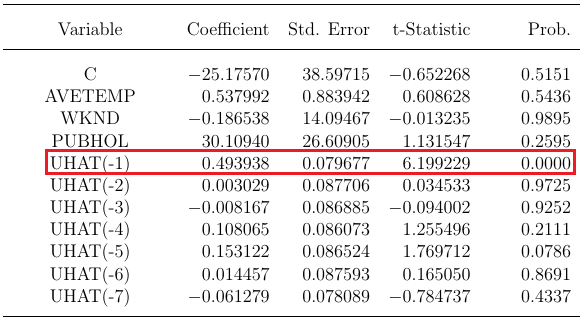
\includegraphics{tute10_16}}
	\end{figure}
	\vspace{-\baselineskip}
	
	\item Correlogram shows that 1st partial autocorrelation is statistically significant, with 4th partial autocorrelation also closely statistically significant
	\item Start by adding an AR(1) error in the model of $aveload$, \begin{align*}
	aveload_t &= \beta_0 + \beta_1 avetemp_t + \beta_2wknd_t + \beta_3pubhol_t + u_t \\
	u_t &= \rho_1u_{t-1} + e_t
	\end{align*} then estimate this model and check the residual correlogram to see if there is a need to consider a higher order AR model for the errors (you could also inspect the residual plot to see if the amended model adequately captures the dynamics of errors).
\end{itemize} 

\newpage
\noindent To estimate model of $aveload$ with an AR(1) error \begin{align*}
aveload_t &= \beta_0 + \beta_1 avetemp_t + \beta_2wknd_t + \beta_3pubhol_t + u_t \\
u_t &= \rho_1u_{t-1} + e_t
\end{align*} in EViews, $$Quick \to Estimate\ Equation$$
\begin{figure}[H]
	\centerline{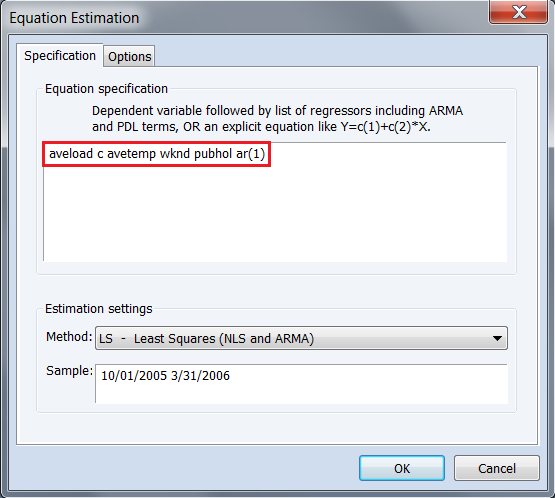
\includegraphics{tute10_11}}
\end{figure}
\vspace{-\baselineskip} then under the $Options$ tab, $$ARMA\ Method:CLS$$ \noindent \textit{A note from the Tutorial 10 Section in Moodle: Different versions of EViews have different default settings for FGLS estimation of a model with AR errors. Therefore, you may get results that are slightly different from the results given in the answer key depending on the version of EViews that you are using. However, the qualitative conclusions will be the same even if the estimates slightly differ numerically.}
\begin{figure}[H]
	\centerline{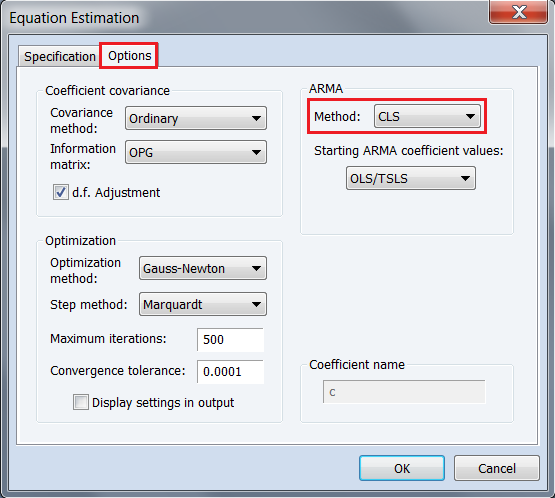
\includegraphics{tute10_12}}
\end{figure}
\vspace{-\baselineskip} 
%%%%%%%%%% TABLE OBJECT %%%%%%%%%%
\begin{table}[H]
	\centering
	\begin{tabular}{lrrrr}
		\multicolumn{3}{l}{Dependent Variable: AVELOAD}&\multicolumn{1}{c}{}&\multicolumn{1}{c}{}\\
		\multicolumn{5}{l}{Method: ARMA Conditional Least Squares (Gauss-Newton / Marquardt}\\
		\multicolumn{2}{l}{steps)}&\multicolumn{1}{c}{}&\multicolumn{1}{c}{}&\multicolumn{1}{c}{}\\
		\multicolumn{4}{l}{Sample (adjusted): 10/02/2005 3/31/2006}&\multicolumn{1}{c}{}\\
		\multicolumn{5}{l}{Included observations: 181 after adjustments}\\
		\multicolumn{5}{l}{Convergence achieved after 12 iterations}\\
		\multicolumn{5}{l}{Coefficient covariance computed using outer product of gradients}\\
		[4.5pt] \hline \\ [-4.5pt]
		\multicolumn{1}{c}{Variable}&\multicolumn{1}{r}{Coefficient}&\multicolumn{1}{r}{Std. Error}&\multicolumn{1}{r}{t-Statistic}&\multicolumn{1}{r}{Prob.}\\
		[4.5pt] \hline \\ [-4.5pt]
		\multicolumn{1}{c}{C}&\multicolumn{1}{r}{$3582.213$}&\multicolumn{1}{r}{$85.97658$}&\multicolumn{1}{r}{$41.66498$}&\multicolumn{1}{r}{$0.0000$}\\
		\multicolumn{1}{c}{AVETEMP}&\multicolumn{1}{r}{$-26.35015$}&\multicolumn{1}{r}{$1.466074$}&\multicolumn{1}{r}{$-17.97327$}&\multicolumn{1}{r}{$0.0000$}\\
		\multicolumn{1}{c}{WKND}&\multicolumn{1}{r}{$-146.2892$}&\multicolumn{1}{r}{$10.02363$}&\multicolumn{1}{r}{$-14.59443$}&\multicolumn{1}{r}{$0.0000$}\\
		\multicolumn{1}{c}{PUBHOL}&\multicolumn{1}{r}{$-48.19995$}&\multicolumn{1}{r}{$19.12197$}&\multicolumn{1}{r}{$-2.520658$}&\multicolumn{1}{r}{$0.0126$}\\
		\multicolumn{1}{c}{AR(1)}&\multicolumn{1}{r}{$0.914550$}&\multicolumn{1}{r}{$0.030277$}&\multicolumn{1}{r}{$30.20613$}&\multicolumn{1}{r}{$0.0000$}\\
		[4.5pt] \hline \\ [-4.5pt]
		\multicolumn{1}{l}{R-squared}&\multicolumn{1}{r}{$0.965152$}&\multicolumn{2}{l}{Mean dependent var}&\multicolumn{1}{r}{$2390.249$}\\
		\multicolumn{1}{l}{Adjusted R-squared}&\multicolumn{1}{r}{$0.964360$}&\multicolumn{2}{l}{S.D. dependent var}&\multicolumn{1}{r}{$362.3839$}\\
		\multicolumn{1}{l}{S.E. of regression}&\multicolumn{1}{r}{$68.41268$}&\multicolumn{2}{l}{Akaike info criterion}&\multicolumn{1}{r}{$11.31623$}\\
		\multicolumn{1}{l}{Sum squared resid}&\multicolumn{1}{r}{$823732.0$}&\multicolumn{2}{l}{Schwarz criterion}&\multicolumn{1}{r}{$11.40459$}\\
		\multicolumn{1}{l}{Log likelihood}&\multicolumn{1}{r}{$-1019.119$}&\multicolumn{2}{l}{Hannan-Quinn criter.}&\multicolumn{1}{r}{$11.35205$}\\
		\multicolumn{1}{l}{F-statistic}&\multicolumn{1}{r}{$1218.633$}&\multicolumn{2}{l}{Durbin-Watson stat}&\multicolumn{1}{r}{$2.183122$}\\
		\multicolumn{1}{l}{Prob(F-statistic)}&\multicolumn{1}{r}{$0.000000$}&\multicolumn{1}{c}{}&\multicolumn{1}{c}{}&\multicolumn{1}{c}{}\\
		[4.5pt] \hline \\ [-4.5pt]
		\multicolumn{1}{l}{Inverted AR Roots}&\multicolumn{1}{l}{.91}&\multicolumn{1}{c}{}&\multicolumn{1}{c}{}&\multicolumn{1}{c}{}\\
		[4.5pt] \hline \\ [-4.5pt]
	\end{tabular}
	\begin{align*}
	{aveload}_t &= \underset{(85.9766)}{3582.213} - \underset{(1.4661)}{26.3502}avetemp_t - \underset{(10.0236)}{146.2892}wknd_t - \underset{(19.1220)}{48.2000}pubhol_t  + \hat{u}_t \\
	\hat{u}_t &= \underset{(0.0303)}{0.9146}\hat{u}_{t-1} + \hat{e}_t \qquad R^2 = 0.9652
	\end{align*} \noindent Note the way that the estimated model is reported when incorporating AR errors.
\end{table} \vspace{-\baselineskip} \noindent To obtain the correlogram of the residual of the estimated $aveload$ model with AR(1) errors (I've named this equation eq03), $$eq03 \to View \to Residual\ Diagnostics \to Correlogram\ Q-statistics$$ \begin{figure}[H]
\centerline{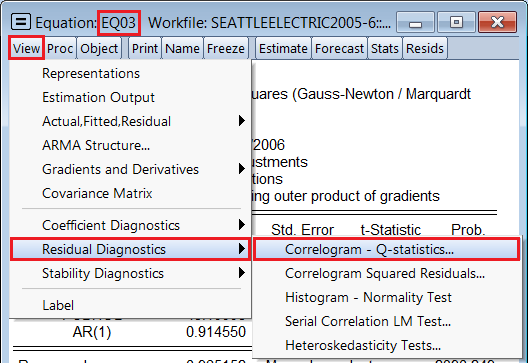
\includegraphics{tute10_13}}
\end{figure}
\vspace{-\baselineskip} $$Lags\ to\ include:36$$ \begin{figure}[H]
	\centerline{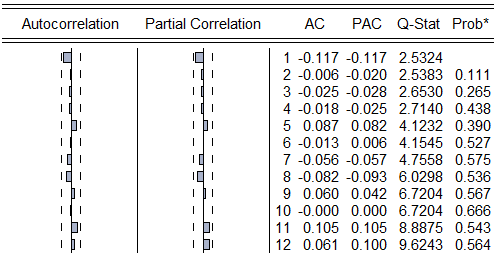
\includegraphics{tute10_14}}
\end{figure}
\vspace{-\baselineskip} \noindent We can check for evidence of serial correlation in the errors by inspecting the correlogram from the residuals. If the sample autocorrelation coefficients are within the significance bands, then they are not statistically significantly different from 0, which would suggest that there is insufficient evidence of serial correlation in the errors.

\noindent As we can see from the correlogram of the residuals, all the sample autocorrelation coefficients lie within the significance bands $\therefore$ there is insufficient evidence to suggest that the errors are serially correlated so the regression with AR(1) errors has taken care of serial correlation in the errors.

\noindent This means that the model of $aveload$ with AR(1) errors does not have serially correlated errors.

\noindent Notes about the estimates of the parameters in the $aveload$ model with AR(1) errors:
\begin{itemize}
	\item The feasible generalised least squares (FGLS) estimator is used to estimate this parameters.
	\item Since the parameters are non-linear (see page 20-22 of Week 9 lecture notes for derivation of model), the FGLS is not unbiased.
	\item FGLS is consistent which means that as the sample size increases, the FGLS estimator converges to the parameter (it converges to the truth).
	\item In large samples, the FGLS estimator is more efficient that the OLS estimator.
	\item Hypothesis tests based on the FGLS standard errors are valid when the sample is large (i.e. asymptotically valid).
\end{itemize}






\newpage
\noindent \textcolor{red}
{
	(e) Using the regression model with AR errors, investigate if the sensitivity of electricity load to temperature (i.e. the coefficient of temperature) is different in weekends relative to the rest of the week.
}

\noindent If we suspect that the sensitivity of electricity load to temperature is different in weekends relative to the rest of the week then we should include the interaction term $$wknd_t\times avetemp_t$$ in our regression model of $aveload$, $$aveload_t = \beta_0 + \beta_1 avetemp_t + \beta_2wknd_t + \beta_3pubhol_t + \beta_4wknd_t\times avetemp_t + u_t$$ Taking the partial derivative of $aveload_t$ with respect to $avetemp_t$ gives the partial effect of $avetemp_t$ on $aveload_t$: $$\dfrac{\partial aveload_t}{\partial avetemp_t} = \beta_1 + \beta_4 wknd_t$$ that is, it is an equation that describes the effects of temperature on electricity load holding the other variables constant. 

\noindent The effect on electricity load for a 1 Fahrenheit degree increase in temperature during the weekend (and holding public holiday constant) is given by, $$\beta_1 + \beta_4$$ while the effect on electricty load for a 1 Fahrenheit degree increase in temperature during the weekday (and holding public holiday constant) is given by, $$\beta_1$$ As such, if the effect of temperature on electricity is not different between weekends and weekdays then the coefficient $\beta_4$ equals to 0, $$H_0: \beta_4 = 0$$ but if there is a difference then, $$H_1: \beta_4 \neq 0$$

\newpage
\noindent To estimate model of $aveload$ with an AR(1) error and with the interaction term $wknd_t\times pubhol_t$ \begin{align*}
aveload_t &= \beta_0 + \beta_1 avetemp_t + \beta_2wknd_t + \beta_3pubhol_t + \beta_4wknd_t\times pubhol_t + u_t \\
u_t &= \rho_1u_{t-1} + e_t
\end{align*} in EViews, $$Quick \to Estimate\ Equation$$
\begin{figure}[H]
	\centerline{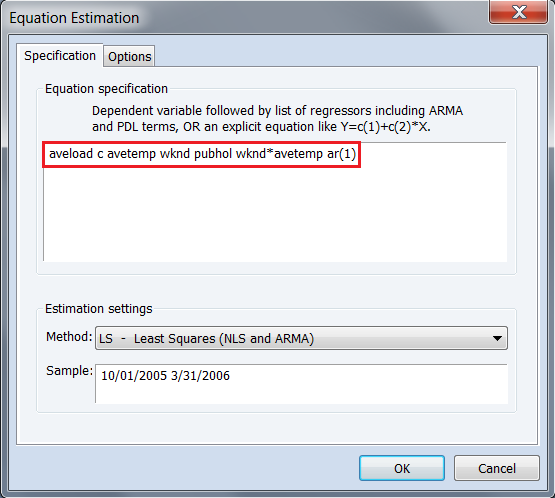
\includegraphics{tute10_15}}
\end{figure}
\vspace{-\baselineskip} then under the $Options$ tab, choose $ARMA\ Method:CLS$
\begin{figure}[H]
	\centerline{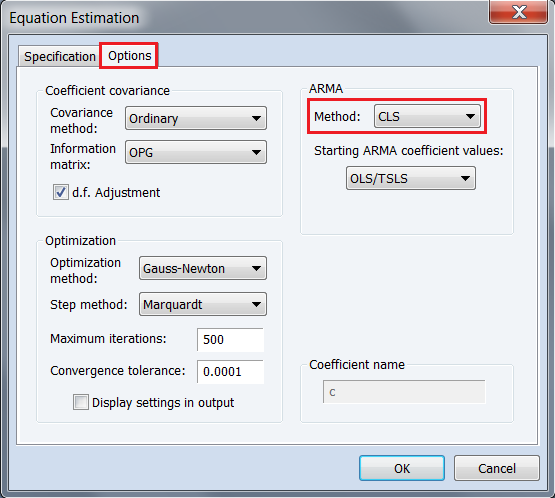
\includegraphics{tute10_12}}
\end{figure}
\vspace{-\baselineskip} \noindent \textit{A note from the Tutorial 9 tab in Moodle: Different versions of EViews have different default settings for FGLS estimation of a model with AR errors. Therefore, you may get results that are slightly different from the results given in the answer key depending on the version of EViews that you are using. However, the qualitative conclusions will be the same even if the estimates slightly differ numerically.}
%%%%%%%%%% TABLE OBJECT %%%%%%%%%%
\begin{table}[H]
	\centering
	\begin{tabular}{lrrrr}
		\multicolumn{3}{l}{Dependent Variable: AVELOAD}&\multicolumn{1}{c}{}&\multicolumn{1}{c}{}\\
		\multicolumn{5}{l}{Method: ARMA Conditional Least Squares (Gauss-Newton / Marquardt}\\
		\multicolumn{2}{l}{steps)}&\multicolumn{1}{c}{}&\multicolumn{1}{c}{}&\multicolumn{1}{c}{}\\
		\multicolumn{3}{l}{Date: 10/01/18   Time: 22:00}&\multicolumn{1}{c}{}&\multicolumn{1}{c}{}\\
		\multicolumn{4}{l}{Sample (adjusted): 10/02/2005 3/31/2006}&\multicolumn{1}{c}{}\\
		\multicolumn{5}{l}{Included observations: 181 after adjustments}\\
		\multicolumn{5}{l}{Convergence achieved after 13 iterations}\\
		\multicolumn{5}{l}{Coefficient covariance computed using outer product of gradients}\\
		[4.5pt] \hline \\ [-4.5pt]
		\multicolumn{1}{c}{Variable}&\multicolumn{1}{r}{Coefficient}&\multicolumn{1}{r}{Std. Error}&\multicolumn{1}{r}{t-Statistic}&\multicolumn{1}{r}{Prob.}\\
		[4.5pt] \hline \\ [-4.5pt]
		\multicolumn{1}{c}{C}&\multicolumn{1}{r}{$3575.808$}&\multicolumn{1}{r}{$87.10534$}&\multicolumn{1}{r}{$41.05153$}&\multicolumn{1}{r}{$0.0000$}\\
		\multicolumn{1}{c}{AVETEMP}&\multicolumn{1}{r}{$-26.21469$}&\multicolumn{1}{r}{$1.494040$}&\multicolumn{1}{r}{$-17.54617$}&\multicolumn{1}{r}{$0.0000$}\\
		\multicolumn{1}{c}{WKND}&\multicolumn{1}{r}{$-118.7532$}&\multicolumn{1}{r}{$56.30826$}&\multicolumn{1}{r}{$-2.108984$}&\multicolumn{1}{r}{$0.0364$}\\
		\multicolumn{1}{c}{PUBHOL}&\multicolumn{1}{r}{$-48.73944$}&\multicolumn{1}{r}{$19.19379$}&\multicolumn{1}{r}{$-2.539333$}&\multicolumn{1}{r}{$0.0120$}\\
		\multicolumn{1}{c}{WKND*AVETEMP}&\multicolumn{1}{r}{$-0.632066$}&\multicolumn{1}{r}{$1.271752$}&\multicolumn{1}{r}{$-0.497004$}&\multicolumn{1}{r}{$0.6198$}\\
		\multicolumn{1}{c}{AR(1)}&\multicolumn{1}{r}{$0.914551$}&\multicolumn{1}{r}{$0.030417$}&\multicolumn{1}{r}{$30.06718$}&\multicolumn{1}{r}{$0.0000$}\\
		[4.5pt] \hline \\ [-4.5pt]
		\multicolumn{1}{l}{R-squared}&\multicolumn{1}{r}{$0.965201$}&\multicolumn{2}{l}{Mean dependent var}&\multicolumn{1}{r}{$2390.249$}\\
		\multicolumn{1}{l}{Adjusted R-squared}&\multicolumn{1}{r}{$0.964207$}&\multicolumn{2}{l}{S.D. dependent var}&\multicolumn{1}{r}{$362.3839$}\\
		\multicolumn{1}{l}{S.E. of regression}&\multicolumn{1}{r}{$68.55950$}&\multicolumn{2}{l}{Akaike info criterion}&\multicolumn{1}{r}{$11.32587$}\\
		\multicolumn{1}{l}{Sum squared resid}&\multicolumn{1}{r}{$822570.9$}&\multicolumn{2}{l}{Schwarz criterion}&\multicolumn{1}{r}{$11.43190$}\\
		\multicolumn{1}{l}{Log likelihood}&\multicolumn{1}{r}{$-1018.991$}&\multicolumn{2}{l}{Hannan-Quinn criter.}&\multicolumn{1}{r}{$11.36885$}\\
		\multicolumn{1}{l}{F-statistic}&\multicolumn{1}{r}{$970.7848$}&\multicolumn{2}{l}{Durbin-Watson stat}&\multicolumn{1}{r}{$2.186007$}\\
		\multicolumn{1}{l}{Prob(F-statistic)}&\multicolumn{1}{r}{$0.000000$}&\multicolumn{1}{c}{}&\multicolumn{1}{c}{}&\multicolumn{1}{c}{}\\
		[4.5pt] \hline \\ [-4.5pt]
		\multicolumn{1}{l}{Inverted AR Roots}&\multicolumn{1}{l}{.91}&\multicolumn{1}{c}{}&\multicolumn{1}{c}{}&\multicolumn{1}{c}{}\\
		[4.5pt] \hline \\ [-4.5pt]
	\end{tabular}
	\begin{align*}
	{aveload}_t &= \underset{(87.1053)}{3575.808} - \underset{(1.4940)}{26.32147}avetemp_t - \underset{(56.3083)}{118.7532}wknd_t - \underset{(19.1938)}{48.7394}pubhol_t \\
	&- \underset{(1.2718)}{0.6321}wknd\times avetemp_t + \hat{u}_t \\
	\hat{u}_t &= \underset{(0.0304)}{0.9146}\hat{u}_{t-1} + \hat{e}_t \qquad R^2 = 0.9652
	\end{align*} \justify \noindent Note the way that the estimated model is reported when incorporating AR errors.
	\begin{align*}
	H_0&: \beta_4 = 0 \\
	H_1&: \beta_4 \neq 0 
	\end{align*} $$p-value=0.6198$$
	\justify \noindent There is insufficient evidence from our sample to suggest that the sensitivity electricity load to temperature differs between weekends and weekdays.
\end{table}



\newpage
\noindent \textcolor{red}
{
	(f) Using the regression model with AR errors, investigate if having dummies for Saturday and Sunday separately instead of $wknd$ would improve the model. In other words, test the hypothesis $H_0: \beta_{SAT} = \beta_{SUN}$.
}
\begin{align*}
	aveload_t &= \beta_0 + \beta_1 avetemp_t + \beta_2pubhol_t + \beta_{SAT}sat_t + \beta_{SUN}sun_t + u_t \\
	u_t &= \rho u_{t-1} + e_t
\end{align*}
$$OR$$
\begin{align*}
aveload_t &= \beta_0 + \beta_1 avetemp_t + \beta_2pubhol_t + \beta_{WKND}wknd_t\\
u_t &= \rho u_{t-1} + e_t
\end{align*}

\noindent The null hypothesis that $\beta_{SAT} = \beta_{SUN}$ suggests that the difference in average electricity usage between Saturday the weekdays is the same as the difference in average electricity usage between Sunday and the weekdays (since Sat and Sun dummies are included as regressors, weekday is the base dummy variable) i.e. that on either days of the weekend average electricity usage differs from the weekday by the same amount.

\noindent Imposing the restriction,
$$\beta_{SAT} = \beta_{SUN}$$
\noindent we have, 
\begin{align*}
aveload_t &= \beta_0 + \beta_1 avetemp_t + \beta_2pubhol_t + \beta_{SAT}sat_t + \boldsymbol{\beta_{SAT}}sun_t + u_t \\
&= \beta_0 + \beta_1 avetemp_t + \beta_2pubhol_t + \boldsymbol{\beta_{SAT}}(sat_t + sun_t) + u_t \\
&= \beta_0 + \beta_1 avetemp_t + \beta_2pubhol_t + \boldsymbol{\beta_{SAT}}(wknd_t) + u_t
\end{align*}

\noindent \textbf{Unrestricted model:}
$$aveload_t = \beta_0 + \beta_1 avetemp_t + \beta_2pubhol_t + \beta_{SAT}sat_t + \beta_{SUN}sun_t + u_t$$

\noindent \textbf{Restricted model:}
$$aveload_t = \beta_0 + \beta_1 avetemp_t + \beta_2pubhol_t + \boldsymbol{\beta_{SAT}}wknd_t + u_t$$

\newpage
$H_0:\beta_{SAT} = \beta_{SUN}$ \quad $(restricted\ model)$

$H_1:\beta_{SAT} \neq \beta_{SUN}$ \quad $(unrestricted\ model)$

\noindent To estimate the unrestricted model in EViews,
$$aveload\ c\ avetemp\ pubhol\ sat\ sun\ AR(1)$$
$$ARMA\ Method:CLS$$
%%%%%%%%%% TABLE OBJECT %%%%%%%%%%
\begin{table}[!htbp]
	\centering
	\begin{tabular}{lrrrr}
		\multicolumn{3}{l}{Dependent Variable: AVELOAD}&\multicolumn{1}{c}{}&\multicolumn{1}{c}{}\\
		\multicolumn{5}{l}{Method: ARMA Conditional Least Squares (Gauss-Newton / Marquardt}\\
		\multicolumn{2}{l}{steps)}&\multicolumn{1}{c}{}&\multicolumn{1}{c}{}&\multicolumn{1}{c}{}\\
		\multicolumn{4}{l}{Sample (adjusted): 10/02/2005 3/31/2006}&\multicolumn{1}{c}{}\\
		\multicolumn{5}{l}{Included observations: 181 after adjustments}\\
		\multicolumn{5}{l}{Convergence achieved after 12 iterations}\\
		\multicolumn{5}{l}{Coefficient covariance computed using outer product of gradients}\\
		[4.5pt] \hline \\ [-4.5pt]
		\multicolumn{1}{c}{Variable}&\multicolumn{1}{r}{Coefficient}&\multicolumn{1}{r}{Std. Error}&\multicolumn{1}{r}{t-Statistic}&\multicolumn{1}{r}{Prob.}\\
		[4.5pt] \hline \\ [-4.5pt]
		\multicolumn{1}{c}{C}&\multicolumn{1}{r}{$3574.174$}&\multicolumn{1}{r}{$86.51799$}&\multicolumn{1}{r}{$41.31134$}&\multicolumn{1}{r}{$0.0000$}\\
		\multicolumn{1}{c}{AVETEMP}&\multicolumn{1}{r}{$-26.14050$}&\multicolumn{1}{r}{$1.441350$}&\multicolumn{1}{r}{$-18.13612$}&\multicolumn{1}{r}{$0.0000$}\\
		\multicolumn{1}{c}{PUBHOL}&\multicolumn{1}{r}{$-43.72776$}&\multicolumn{1}{r}{$18.83209$}&\multicolumn{1}{r}{$-2.321981$}&\multicolumn{1}{r}{$0.0214$}\\
		\multicolumn{1}{c}{SAT}&\multicolumn{1}{r}{$-130.6781$}&\multicolumn{1}{r}{$11.43118$}&\multicolumn{1}{r}{$-11.43172$}&\multicolumn{1}{r}{$0.0000$}\\
		\multicolumn{1}{c}{SUN}&\multicolumn{1}{r}{$-160.9819$}&\multicolumn{1}{r}{$11.25608$}&\multicolumn{1}{r}{$-14.30177$}&\multicolumn{1}{r}{$0.0000$}\\
		\multicolumn{1}{c}{AR(1)}&\multicolumn{1}{r}{$0.918613$}&\multicolumn{1}{r}{$0.029535$}&\multicolumn{1}{r}{$31.10215$}&\multicolumn{1}{r}{$0.0000$}\\
		[4.5pt] \hline \\ [-4.5pt]
		\multicolumn{1}{l}{R-squared}&\multicolumn{1}{r}{$0.966522$}&\multicolumn{2}{l}{Mean dependent var}&\multicolumn{1}{r}{$2390.249$}\\
		\multicolumn{1}{l}{Adjusted R-squared}&\multicolumn{1}{r}{$0.965565$}&\multicolumn{2}{l}{S.D. dependent var}&\multicolumn{1}{r}{$362.3839$}\\
		\multicolumn{1}{l}{S.E. of regression}&\multicolumn{1}{r}{$67.24636$}&\multicolumn{2}{l}{Akaike info criterion}&\multicolumn{1}{r}{$11.28719$}\\
		\multicolumn{1}{l}{Sum squared resid}&\multicolumn{1}{r}{$791362.9$}&\multicolumn{2}{l}{Schwarz criterion}&\multicolumn{1}{r}{$11.39322$}\\
		\multicolumn{1}{l}{Log likelihood}&\multicolumn{1}{r}{$-1015.491$}&\multicolumn{2}{l}{Hannan-Quinn criter.}&\multicolumn{1}{r}{$11.33018$}\\
		\multicolumn{1}{l}{F-statistic}&\multicolumn{1}{r}{$1010.449$}&\multicolumn{2}{l}{Durbin-Watson stat}&\multicolumn{1}{r}{$2.114403$}\\
		\multicolumn{1}{l}{Prob(F-statistic)}&\multicolumn{1}{r}{$0.000000$}&\multicolumn{1}{c}{}&\multicolumn{1}{c}{}&\multicolumn{1}{c}{}\\
		[4.5pt] \hline \\ [-4.5pt]
		\multicolumn{1}{l}{Inverted AR Roots}&\multicolumn{1}{l}{.92}&\multicolumn{1}{c}{}&\multicolumn{1}{c}{}&\multicolumn{1}{c}{}\\
		[4.5pt] \hline \\ [-4.5pt]
	\end{tabular}
	%\caption{Add your caption here.}
	%\label{tab:}
\end{table}


\vspace{-\baselineskip}
$$SSR_{ur} = 791362.9$$


\noindent We have estimated the restricted model earlier,
$$SSR_{r} = 823732.0$$
$$F = \dfrac{(SSR_r - SSR_{ur})/q}{SSR_{ur}/(n-k-1)} = \dfrac{(SSR_r - SSR_{ur})/1}{SSR_{ur}/(181-5-1)} \sim F_{1,175} \quad under\ H_0$$
$$F_{calc} = \dfrac{(823732.0 - 791362.9)/1}{791362.9/(175)} = 7.158$$
\noindent To obtain the critical value from the Command window in EViews,
$$scalar\ cv\ = @qfdist(0.95,1,175)$$
\begin{figure}[H]
	\centerline{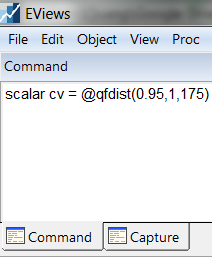
\includegraphics{tute10_17}}
\end{figure}
\vspace{-\baselineskip}
\begin{figure}[H]
	\centerline{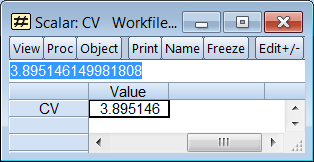
\includegraphics{tute10_18}}
\end{figure}
\vspace{-\baselineskip}
$$F_{crit} = 3.92$$
\noindent Since $F_{calc} = 7.158 > F_{crit} = 3.92$ we reject the null at the 5\% significance level and conclude that there is sufficient evidence from our sample in support for the model with separate dummies of Saturday and Sunday.





\end{document}